\chapter{Correlation effects in attosecond electron dynamics} % (fold)
\label{cha:electron_correlation}

%%%%%%%%%%%%%%%%%%%%%%%%%%%%%%%%%%%%%%%%%%%%%%%%%%%%%%%%%%%%%%%%%%%%%%%%%%%%%%%%%%%%%%%%%%%%%%%%%%%%%%%%%%%%%%%%%%
%%%%%%%%%%%%%%%%%%%%%%%%%%%%%%%%%%%%%%%%%%%%%%%%%%%%%%%%%%%%%%%%%%%%%%%%%%%%%%%%%%%%%%%%%%%%%%%%%%%%%%%%%%%%%%%%%%
%%%%%%%%%%%%%%%%%%%%%%%%%%%%%%%%%%%%%%%%%%%%%%%%%%%%%%%%%%%%%%%%%%%%%%%%%%%%%%%%%%%%%%%%%%%%%%%%%%%%%%%%%%%%%%%%%%
%%%%%%%%%%%%%%%%%%%%%%%%%%%%%%%%%%%%%%%%%%%%%%%%%%%%%%%%%%%%%%%%%%%%%%%%%%%%%%%%%%%%%%%%%%%%%%%%%%%%%%%%%%%%%%%%%%
%%%%%%%%%%%%%%%%%%%%%%%%%%%%%%%%%%%%%%%%%%%%%%%%%%%%%%%%%%%%%%%%%%%%%%%%%%%%%%%%%%%%%%%%%%%%%%%%%%%%%%%%%%%%%%%%%%
\section{Hyperspherical harmonics}
\label{sec:hyperspherical}

Solving the TDSE for two active electrons is a computationally difficult task. A Naive approach would be to discretized the 6 spacial dimensions using finite difference. Finite difference would provide a straight forward solution and runs well on supercomputing systems, however, the size of the wavefunction scales like $N^6$. Therefore if we were to us a typical grid of 1000 points in each dimension, the wavefunction would be $10^{18}$ points in size. Merely writing down the wavefunction in double precision floating point numbers would require 16 Exabytes of RAM, approximately 100 times more RAM than exists on the largest supercomputer in the world (Summit, OLCF). Instead, it is convent to choose a basis that greatly reduces the size of the problem. One common approach is to use bi-spherical harmonics. In this case, each electron is expanded in 3D spherical coordinates. The radius is discretized with finite difference, b-splines, FEDVR, or similar method, and the two angular coordinates are explained in the standard 3D spherical harmonics in the same way a single active electron code would do. When taking the tensor product of the two electrons, the electron-electron repulsion term is then expanded in spherical harmonics such that
\begin{equation}
    \frac{1}{|\mathbf{r}_1-\mathbf{r}_2|}= 4\pi \sum_{\ell=0}^\infty \sum_{m=-\ell}^{m=\ell}\frac{1}{2\ell+1}\frac{r_<^\ell}{r_>^{\ell+1}}Y_{\ell m}^*(\theta_1, \phi_1)Y_{\ell m}^(\theta_2, \phi_2).
\end{equation}
Resulting in a 6D space that can be used to solve the problem of two electrons in a molecular or atomic potential interacting with a laser.

In the bi-spherical codes, one must discretize two radi. As the grid increases in size, the code likes $N^2$. To cercomvent this problem, I have implemented a code that contains a single hyper-radius ($R$) and five angles that are expanded in 6D hyperspherical harmonics. Therefore as the grid size is increased, the code scales like $N$ and the number of spherical harmonics is controlled by the laser parameters. In the following section, I will describe the details to implementing two different ``coordinate systems'' that solve the two active electron problem. The first is through the use of Jacobi Coordinates, which allows for the finite mass of the nucleus to be accounted for. The second is making the infinite mass approximation for the nucleus allowing for the distance between the two electrons to be accessed more directly. The two problems can be solved with similar sized wavefunctions, however, the second method has a greatly reduced time in calculating matrix elements. This section is laid out $\cdots$ \textbf{TODO}

\subsection{TDSE in hyperspherical coordinates} % (fold)
\label{sub:tdse_in_hyperspherical_coordinates}
The TDSE
\begin{equation}
    i\frac{\partial}{\partial t}\Psi = \hat{H}\Psi
\end{equation}
with hamiltonian written in hyperspherical coordinates is
\begin{equation}
   \hat{H} = -\frac{1}{2} \left[\frac{1}{R^5}\frac{\partial}{\partial R}\left(R^5\frac{\partial}{\partial R}\right) - \frac{\hat{K}^2(\Omega_5)}{R^2}\right] + \frac{W(\Omega_5)}{R}
\end{equation}
where $R=\sum_i x_i^2$ is the hyper radius with $x_i$ being a Cartesian coordinate, $\hat{K}$ as the angular momentum operator, $\Omega_5$ is the solid angle in 6D (5 angles), and $V(\mathbf{R}) = W(\Omega_5)/R$ being the potential. I will use the hyperspherical harmonics such they contain two-3D sub spaces as described in Sec.~\ref{ssub:spherical_harmonics}. 
The resulting volume elements are 
\begin{equation}
    d\tau = R^5 dr d\Omega_i
\end{equation}
\begin{equation}
    d\Omega_i = \cos^2\alpha \sin^2\alpha d\alpha d\omega
\end{equation}
\begin{equation}
    d\omega = \sin\theta_{r_1} d\theta_{r_1} d\phi_{r_1} \sin\theta_{r_1} d\theta_{r_1} d\phi_{r_1}
\end{equation}
where $\theta_i$ and $\phi_i$ denote the angles in the $i={r_1}$ and $i={r_1}$ sub coordinate systems and $\alpha$ is the angle produced by the right triangle with sides R, ${r_1}$, and ${r_1}$ as shown in Fig.~\ref{fig:hyperradius}. $r_1$ and $r_2$ will be used as the Jacobi Coordinates for finite mass nucleus is considered or the single electron coordinates when the infinite mass approximation is made.
\begin{figure}[h!]
\centering
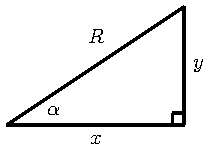
\includegraphics[width=0.3\linewidth]{figs/Two_electron/hyperradius.pdf}
\caption{How the hyperradius (R) relates to the two single-electron sub coordinate systems ($r_1$, $r_2$)} 
  \label{fig:hyperradius}
\end{figure}

As with the 3D TDSE, it is beneficial to remove the first derivative in the radial equation. This is accomplished by making a substitution of $\Psi = \psi/R^{5/2}$ giving us a Hamiltonian
\begin{equation}
   \hat{H} = -\frac{1}{2} \left[\frac{\partial^2}{\partial R^2} - \frac{\hat{K}^2(\Omega_5)+15/4}{R^2}\right] + \frac{W(\Omega_5)}{R}.
\end{equation}
The wavefunction can now be written as
\begin{equation}
    \psi = \sum\limits_{\mathbf{K}} U_{\mathbf{K}}(R) Y_{\mathbf{K}}(\Omega_5)
\end{equation}
with $U_{\mathbf{k}}(R)$ being the hyperradial part of the wavefunction and $Y_{\mathbf{K}}(\Omega_5)$ being the 6D hyperspherical harmonics described in Sec.~\ref{ssub:spherical_harmonics}. Since hyperspherical harmonics are eigenfunctions of $\hat{K}^2$ with eigenvalue $K(K+4)$, the Hamiltonian becomes
\begin{equation}
   \hat{H}_{K} = -\frac{1}{2} \left[\frac{\partial^2}{\partial R^2} - \frac{K(K+4)+15/4}{R^2}\right] + \frac{W(\Omega_5)}{R}.
\end{equation}
I solve this equation using finite difference to discretized the hyperradial function ($U_{\mathbf{K}}(R)$). By setting $W(\Omega_5)=1$, the equation is the 6D hydrogen atom with an analytic solution that can be used to test the hyperadial portion of the code (see \cite{S_revik_2005} for energy levels). The angular portion of the equations is then expanded in hyperspherical harmonics. The details of the expansion are the focus of the remainder of this section.
% subsection tdse_in_hyperspherical_coordinates (end)

\subsubsection{Hyperspherical Harmonic Definition} % (fold)
\label{ssub:spherical_harmonics}
There are multiple ways to define hyperspherical harmonics in 6D. Since they are equivalent up to a unitary rotation, it is best to choose those that match the symetry of the problem. In our case, we choose spherical harmonics that contain a hyperangle $\alpha$ that connects two-3D spaces as shown in Fig.~\ref{fig:hyperradius}. The 3D spaces belong to coordinates $\mathbf{r}_1$ and $\mathbf{r}_2$ with radii $r_1$ and $r_2$ respectively. These spaces will either represent a Jacobi Coordinate (Sec.~\ref{ssub:jacobi_coordinates}) or the space of each electron (Sec.~\ref{ssub:electronic_coordinates}). The resulting 6D spherical harmonics are given by
\begin{align}
    Y^{\ell_{r_1},\ell_{r_2}}_{K,L,M}(\Omega_{5}) =& N^{\ell_{r_1},\ell_{r_2}}_K P_n^{(\ell_{r_1}+1/2,\ell_{r_2}+1/2)}(\cos(2\alpha)) \cos^{\ell_{r_1}}(\alpha) \sin^{\ell_{r_2}}(\alpha) \\ 
    &\times\sum_{m_{r_1},m_{r_2}}\bra{L,M}\ket{\ell_{r_1},m_{r_1},\ell_{r_2},m_{r_2}}  \left[Y_{\ell_{r_1},m_{r_1}}(\hat{r}_1)\times Y_{\ell_{r_2},m_{r_2}}(\hat{r}_2)\right]
\end{align}
with
\begin{equation}
    N^{\ell_{r_1},\ell_{r_2}}_K = \sqrt{\frac{2(K+2)(n!)\Gamma (n+\ell_{r_1}+\ell_{r_2}+2)}{\Gamma (n+\ell_{r_1}+3/2) \Gamma (n+\ell_{r_2}++3/2)}}.
\end{equation}
where $P_n^{(\alpha,\beta)}$ is a Jacobi polynomial, $\bra{L,M}\ket{\ell_{r_1},m_x,\ell_{y_1},m_y}$ is a Clebsch–Gordan coefficient, $\Gamma$ is a gamma function, $Y_{\ell_{r},m_{r}}(\hat{r})$ is the standard 3D spherical harmonics, and $\Omega_5$ is the 6D solid angle containing 5 angular dimensions. $K$, $L$, $M$, $\ell_{r_1}$ and $\ell_{r_2}$ are the quantum numbers with $K=2n+\ell_{x_1}+\ell_{y_1}$ being the grand angular momentum, $\ell_{r_1}\ge0$ and $\ell_{r_2}\ge0$ being the angular momentum for the $\mathbf{r_1}$ and $\mathbf{r_2}$ coordinates respectively, $|\ell_{r_1}-\ell_{r_2}|\le L \le \ell_{r_1}+\ell_{r_2}$ and $-L \le M \le L$. For simplicity, we define $\mathbf{K}=\{K, L, M, \ell_{r_1}, \ell_{r_2}\}$ allowing for the simplified notation $Y_{\mathbf{K}}(\Omega_{5})$.

The hyperspherical harmonics contain three parts, each depending on one free parameter $\alpha$, $\mathbf{r}_1$, and $\mathbf{r}_2$. By defining 
\begin{equation}
    \tilde{P}^{\ell_{r_1},\ell_{r_2}}_{n}(\alpha) = N^{\ell_{r_1},\ell_{r_2}}_K P_n^{(\ell_{r_1}+1/2,\ell_{r_2}+1/2)}(\cos(2\alpha)) \cos^{\ell_{r_1}}(\alpha) \sin^{\ell_{r_2}}(\alpha) 
\end{equation}
hyperspherical harmonics become
\begin{equation}
    Y^{\ell_{r_1},\ell_{r_2}}_{K,L,M}(\Omega_{5}) =\tilde{P}^{\ell_{r_1},\ell_{r_2}}_{n}(\alpha)\sum_{m_{r_1},m_{r_2}}\bra{L,M}\ket{\ell_{r_1},m_{r_1},\ell_{r_2},m_{r_2}}  \left[Y_{\ell_{r_1},m_{r_1}}(\hat{r}_1)\times Y_{\ell_{r_2},m_{r_2}}(\hat{r}_2)\right]
    \label{eq:hyperspherical_harm_simple}
\end{equation}
highlighting the three sections.
% section spherical_harmonics (end)
 
\subsubsection{Jacobi Coordinates} % (fold)
\label{ssub:jacobi_coordinates}
Jacobi coordinates are often used for studying many body interactions. The are defined by choosing a particle and defining a relative coordinated between them. The next particle is defined by a coordinate connecting the center of mass of all the previous particles to the next particle. The result is a set of coordinates that has dimension $3(N-1)$ assuming the exact location of the center of mass $R_{cm}$ in space is irreverent. 
For a three particle system, the center of mass is

\begin{equation}
\mathbf{R_{cm}} = m_1 \mathbf{r_1} + m_2 \mathbf{r_2} + m_3 \mathbf{r_3}
\end{equation}
and three convenient sets of Jacobi coordinates are
\begin{align}
\label{eq:jacobi_coords}
\mathbf{x_1} &= \left[\frac{m_2+m_3}{m_1(m_2+m_3)^2}\right]^{1/4} (\mathbf{r_3}-\mathbf{r_2}); &\mathbf{y_1} &= \left[\frac{m_1(m_2+m_3)^2}{m_2+m_3}\right]^{1/4} \left(\mathbf{r_1}- \frac{m_2\mathbf{r_2}+m_3\mathbf{r_3}}{m_2+m_3} \right)\\
\mathbf{x_2} &= \left[\frac{m_3+m_1}{m_2(m_3+m_1)^2}\right]^{1/4} (\mathbf{r_1}-\mathbf{r_3}); &\mathbf{y_2} &= \left[\frac{m_2(m_3+m_1)^2}{m_3+m_1}\right]^{1/4} \left(\mathbf{r_2}- \frac{m_3\mathbf{r_3}+m_1\mathbf{r_1}}{m_3+m_1} \right)\\
\mathbf{x_3} &= \left[\frac{m_1+m_2}{m_3(m_1+m_2)^2}\right]^{1/4} (\mathbf{r_2}-\mathbf{r_1}); &\mathbf{y_3} &= \left[\frac{m_3(m_1+m_2)^2}{m_1+m_2}\right]^{1/4} \left(\mathbf{r_3}- \frac{m_1\mathbf{r_1}+m_2\mathbf{r_2}}{m_1+m_2} \right).
\end{align}
The three coordinate systems are depicted in Fig.~\ref{fig:jacobi_coord}. For the Helium atom we place the nucleus as $m_1$ and the two electrons at $m_2$ and $m_3$. The we set $m_1\rightarrow \infty$ and $m_2=m_3=m$. Now we define $\beta_i$ with $i=1,2,3$ such that
\begin{align}
\mathbf{x_1} &= \beta_1 (\mathbf{r_3}-\mathbf{r_2}); \; \; \mathbf{y_1} = \frac{1}{\beta_1} \left(\mathbf{r_1}- \frac{\mathbf{r_2}+\mathbf{r_3}}{2} \right)\\
\mathbf{x_2} &= \beta_2 (\mathbf{r_1}-\mathbf{r_3}); \; \; \mathbf{y_2} = \frac{1}{\beta_2} \left(\mathbf{r_2}- \frac{\mathbf{r_3}+\mathbf{r_1}}{2} \right)\\
\mathbf{x_3} &= \beta_3 (\mathbf{r_2}-\mathbf{r_1}); \; \; \mathbf{y_3} = \frac{1}{\beta_2} \left(\mathbf{r_3}- \frac{\mathbf{r_1}+\mathbf{r_2}}{2} \right)
\end{align}
Within the infinite mass approximation, $\beta_1=1/\sqrt{2}$ and $\beta_2=\beta_3=1$. By applying a Raynal-Revai Coefficient (RRC) it is possible to transition between the three different coordinate systems.  The transformation conserves the angular momentum quantum numbers $K$ , $L$, and $M$ of the hyperspherical harmonics.

\begin{figure}[h!]
\centering
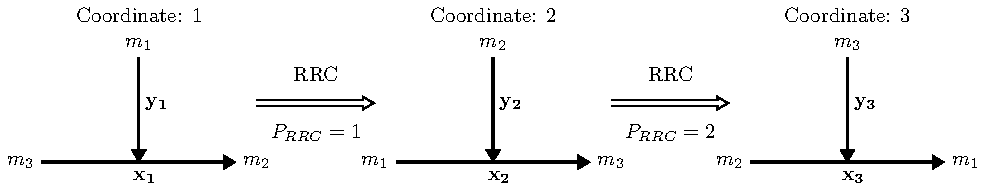
\includegraphics[width=\linewidth]{figs/Two_electron/coord_1.pdf}
\caption{The Jacobi coordinates for three body interactions. Each coordinate can be obtained from the previous by utilizing a Raynal-Revai Coefficient} 
  \label{fig:jacobi_coord}
\end{figure}

The RRC coefficients for rotating between coordinate system $i$ and $j$ can be written explicitly as
\begin{align}
\nonumber
    <\ell_{x_j},\ell_{y_j}|\ell_{x_i},\ell_{y_i}>_{K,L} =& \frac{(-1)^{n_i+n_j}}{\sqrt{C_{\ell_{x_j}\ell_{y_j}}^{n_j}C_{\ell_{x_i}\ell_{y_i}}^{n_i}}} \sum\limits_{\lambda_1,\lambda_2,\lambda_3,\lambda_4} i^{\lambda_2-\lambda_1+\ell_{y_i}-\ell_{y_j}}\left[\prod_{k=1}^4 (2\lambda_k +1)\right] \\ 
\nonumber
    & \times \braket{\lambda_1 0 \lambda_3 0}{\ell_{x_j} 0} \braket{\lambda_2 0 \lambda_3 0}{\ell_{x_i} 0} \braket{\lambda_2 0 \lambda_4 0}{\ell_{y_j} 0} \braket{\lambda_1 0 \lambda_4 0}{\ell_{y_i} 0} \\
\nonumber
    & \times sgn(a_{12})^{\lambda_1}sgn(a_{21})^{\lambda_2}sgn(a_{11})^{\lambda_3}sgn(a_{22})^{\lambda_4} \begin{bmatrix}
   \lambda_3 & \lambda_1 & \ell_{x_j} \\
   \lambda_2 & \lambda_4 & \ell_{y_j} \\
   l_{x_i}   & l_{x_y}   & L
   \end{bmatrix} \\
    & \times \sum\limits_{\nu,\mu} (-1)^{\mu}|a_{12}|^{2\mu + \lambda_1 + \lambda_2} |a_{12}|^{2\nu + \lambda_3 + \lambda_4} C_{\lambda_1 \lambda_2}^{\mu} C_{\lambda_3 \lambda_4}^{\nu}
    \label{eq:RRC}
\end{align}
where $sgn(a_{ij})$ is the sign of $a_{ij}$, the sum is restricted by $K=2n_i+\ell_{x_i}+\ell_{y_i}=2n_j+\ell_{x_j}+\ell_{y_j}=2(\mu+\nu)+\lambda_1+\lambda_2+\lambda_3+\lambda_4$, $\braket{\lambda_1 0 \lambda_3 0}{\ell_{x_j} 0}$ is a Clebsch Gordan coefficient,
     $\begin{bmatrix}
        \lambda_3 & \lambda_1 & \ell_{x_j} \\
        \lambda_2 & \lambda_4 & \ell_{y_j} \\
        l_{x_i}   & l_{x_y}   & L
        \end{bmatrix}$
is a wigner 9j symbol, 
    $C_{\alpha\beta}^\mu = \frac{(2\mu+\alpha+\beta+1)!}{(\mu)!(\mu+\alpha+\beta+1)!(2(\mu+\alpha)+1)!!(2(\mu+\beta)+1)!!}$,
$a_{11} = \cos(\xi_{ki})$,
$a_{22} = \cos(\xi_{ki})$,
$a_{12} = \sin(\xi_{ki})$, and 
$a_{21} = -\sin(\xi_{ki})$
with $\xi_{ki} = \arctan((-1)^{P_{RRC}}\sqrt{Mm_j/(m_i m_k)})$ where $m_i$ is the mass of the ith particle, M is the total mass and $P$ is the number of permutations of $m_1\rightarrow m_2\rightarrow m_3\rightarrow m_1$  as shown in Fig.~\ref{fig:jacobi_coord}. As the value of $K$ increases, RRC become extremely computationally expensive limiting the usefulness of this approach.

\textbf{Should I include this?: Note that this formalism is subject to roundoff error for large values of $K$. When large $K$ is utilized, a recursion relation version should be utilized (see S.\ N.\ Ershov. Nuclei Theory \textbf{79}, 694-702 (2016)).}

Utilizing the Jacobi coordinates 1 in Fig.~\ref{fig:jacobi_coord}, the Helium potential becomes
\begin{equation}
    V(\mathbf{R}) = \frac{1}{r_{23}} - \frac{Z}{r_{12}} - \frac{Z}{r_{13}}
\end{equation}
which can be rewritten as 
\begin{equation}
    W(\Omega_5) = R V(\mathbf{R}) = \frac{\beta_1}{x_1} - \frac{Z}{|\beta_1\hat{y}_1+\hat{x}_1/(2\beta_1)|} - \frac{Z}{|\beta_1\hat{y}_1-\hat{x}_1/(2\beta_1)|}.
\end{equation}
By using the hyperspherical harmonics defined in eq.~\ref{eq:hyperspherical_harm_simple}, with $\mathbf{r_1}=\mathbf{x_1}$ and $\mathbf{r_2}=\mathbf{y_1}$, the first term is easy to calculate through a 1D integral over $\alpha$ written explicitly bellow. However, the next two terms would require a 5D integral which is expensive and numerically unstable if computed directly. Instead, we will exchange particles in the coordinate system to allow the $\mathbf{x}_i$ Jacobi coordinate to correspond to the distance between the two interacting particles. The result is a 1D integral over $\alpha$ that is similar to the $e^-e^-$ repulsion term. To achieve this, we utilize RRC (eq.~\ref{eq:RRC}) which allow us to write
\begin{equation}
    Y^{\ell_{x_i},\ell_{y_i}}_{K,L,M} = \sum\limits_{\ell_{x_j}\ell_{y_j}} <\ell_{x_j},\ell_{y_j}|\ell_{x_i},\ell_{y_i}>_{K,L} Y^{\ell_{x_j},\ell_{y_j}}_{K,L,M}(\Omega_{5_j})
\end{equation}
where $\Omega_{5_i}$ and $\Omega_{5_j}$ are the solid angles in the Jacobi coordinates labeled by $i,j$. We note that $K$, $L$ and $M$ are conserved in this rotation allowing us to remove any subscripts. 

For practical reasons, we need to calculate the matrix elements $\bra{\mathbf{K}'}V(R=1,\Omega_{5_i})\ket{\mathbf{K}} = \bra{\mathbf{K}'}W(\Omega_{5_i})\ket{\mathbf{K}}$ as the term $1/R$ can be factored out of $V(R,\Omega_{5_i})$ removing its dependence on $R$. We can then store the results of $\bra{\mathbf{K}'}W(\Omega_{5_i})\ket{\mathbf{K}}$ in a hash table to be looked up when building the matrix. \textbf{TODO: Cite M. A. Kahn et. al. \textbf{8} 469 (1999)}

The electron electron repulsion term of $W(\Omega_5)$ becomes
\begin{align}
    \bra{K'\ell_{x_1}'\ell_{y_1}'L'M'} \frac{1}{\sqrt{2}\cos\alpha_1} \ket{K \ell_{x_1} \ell_{y_1}LM} =& \frac{1}{\sqrt{2}} \delta_{\ell_{x_1}',\ell_{x_1}} \delta_{\ell_{y_1}',\ell_{y_1}} \delta_{L',L} \delta_{M',M} \\
    & \times \int\limits_0^{\pi/2}\ \tilde{P}^{\ell_{x_1}',\ell_{y_1}'}_{n'}(\alpha_1) \tilde{P}^{\ell_{x_1},\ell_{y_1}}_{n}(\alpha_1) \sin^2(\alpha_1) \cos(\alpha_1)d\alpha_1  
\end{align}
where the delta functions come from the integral over $d\omega$.

The coulomb potential for the $m_3$ electron of $W(\Omega_5)$ becomes
\begin{align}
    \bra{K'\ell_{x_1}'\ell_{y_1}'L'M'} R\frac{-Z}{r_{13}} \ket{K \ell_{x_1} \ell_{y_1}LM} = \sum_{\ell_{x_2},\ell_{y_2}}& <\ell_{x_2},\ell_{y_2}|\ell_{x_1}',\ell_{x_1}'>_{K',L'} <\ell_{x_2},\ell_{y_2}|\ell_{x_1},\ell_{x_1}>_{K,L} \\
    &\times \bra{K'\ell_{x_2}'\ell_{y_2}'L'M'} \frac{-Z}{\cos\alpha_2} \ket{K\ell_{x_2}\ell_{y_2}LM}
\end{align}
with $P_{RRC}=1$  and 
\begin{align}
    \bra{K'\ell_{x_2}'\ell_{y_2}'L'M'} \frac{1}{\sqrt{2}\cos\alpha_2} \ket{K \ell_{x_2} \ell_{y_2}LM} =& \frac{1}{\sqrt{2}} \delta_{\ell_{x_2}',\ell_{x_2}} \delta_{\ell_{y_2}',\ell_{y_2}} \delta_{L',L} \delta_{M',M} \\
    & \times \int\limits_0^{\pi/2}\ \tilde{P}^{\ell_{x_2}',\ell_{y_2}'}_{n'}(\alpha_2) \tilde{P}^{\ell_{x_2},\ell_{y_2}}_{n}(\alpha_2) \sin^2(\alpha_2) \cos(\alpha_2)d\alpha_2  
\end{align}
and the coulomb potential for the $m_2$ electron of $W(\Omega_5)$ becomes
\begin{align}
    \bra{K'\ell_{x_1}'\ell_{y_1}'L'M'} R\frac{-Z}{r_{12}} \ket{K \ell_{x_1} \ell_{y_1}LM} = \sum_{\ell_{x_3},\ell_{y_3}}& <\ell_{x_3},\ell_{y_3}|\ell_{x_1}',\ell_{x_1}'>_{K',L'} <\ell_{x_3},\ell_{y_3}|\ell_{x_1},\ell_{x_1}>_{K,L} \\
    &\times \bra{K'\ell_{x_3}'\ell_{y_3}'L'M'} \frac{-Z}{\cos\alpha_3} \ket{K\ell_{x_3}\ell_{y_3}LM}
\end{align}
with $P_{RRC}=2$  and 
\begin{align}
    \bra{K'\ell_{x_3}'\ell_{y_3}'L'M'} \frac{1}{\sqrt{2}\cos\alpha_3} \ket{K \ell_{x_3} \ell_{y_3}LM} =& \frac{1}{\sqrt{2}} \delta_{\ell_{x_3}',\ell_{x_3}} \delta_{\ell_{y_3}',\ell_{y_3}} \delta_{L',L} \delta_{M',M} \\
    & \times \int\limits_0^{\pi/2}\ \tilde{P}^{\ell_{x_3}',\ell_{y_3}'}_{n'}(\alpha_3) \tilde{P}^{\ell_{x_3},\ell_{y_3}}_{n}(\alpha_3) \sin^2(\alpha_3) \cos(\alpha_3)d\alpha_3.  
\end{align}

Next, the laser potential for a linearly polarized laser aligned along the lab's $z$-axis needs to be calculated. The potential term is
\begin{equation}
     V_{las}(\mathbf{R}) = - E_z z_2 - E_z z_3 = - 2E_z \frac{z_2 + z_3}{2}.
\end{equation} 
where $z_2$ and $z_3$ are the z components of the two electrons and $E_z$ is the magnitude of the $z$ component of the electric field.
Therefore the laser couples to the z component of the center of mass of the two electrons namely
\begin{equation}
    \mathbf{r}_{2e_{cm}} = \frac{\mathbf{r}_2 + \mathbf{r}_3}{2}.
\end{equation}
Noticing that $y_1$ from Eq.~\ref{eq:jacobi_coords} contains $\mathbf{r}_{2e_{cm}}$, the laser term only appears in the $\hat{y}_1$ spherical harmonics. 
Now we need to calculate the $V_{las}(\mathbf{R})$ matrix element such that
\begin{equation}
    \bra{K'\ell_{x_1}'\ell_{y_1}'L'M'} -2E_z z_{2e_{cm}} \ket{K \ell_{x_1} \ell_{y_1}LM}.
\end{equation} 
In the infinite mass approximation, $\mathbf{R_{cm}}=\mathbf{r}_i$  and therefore 
\begin{align}
z_{2e_{cm}}&=\beta_1 \mathbf{y}_1\cdot\hat{z}_{cm} \\
&= \frac{y_1\cos(\theta_{y_1})}{\sqrt{2}}\\
&= 2 \sqrt{\frac{\pi}{6}}y_1Y_{1,0}(\hat{y}_1)\\
&= 2 \sqrt{\frac{\pi}{6}}Rsin(\alpha_1)Y_{1,0}(\hat{y}_1)
\end{align}
Plugging this in we obtain 
\begin{equation}
    \bra{K'\ell_{x_1}'\ell_{y_1}'L'M'}  -2E_z z_{2e_{cm}} \ket{K \ell_{x_1} \ell_{y_1}LM} =-2E_z \bra{K'\ell_{x_1}'\ell_{y_1}'L'M'} 2\sqrt{\frac{\pi}{6}}Rsin(\alpha_1)Y_{1,0}(\hat{y}_1) \ket{K \ell_{x_1} \ell_{y_1}LM} 
\end{equation}
which becomes
\begin{align}
    \nonumber\bra{K'\ell_{x_1}'\ell_{y_1}'L'M'} -2E_z z_{2e_{cm}} \ket{K \ell_{x_1} \ell_{y_1}LM} &= -2E_z\delta_{\ell_{x_1}'\ell_{x_1}} \delta_{M'M} R  \sqrt{\frac{(2\ell_{y_1}'+1)}{2(2\ell_{y_1}+1)}}\\\nonumber
    & \times \left[\int\limits_0^{\pi/2}\ \tilde{P}^{\ell_{x_1}',\ell_{y_1}'}_{n'}(\alpha_1) \tilde{P}^{\ell_{x_1},\ell_{y_1}}_{n}(\alpha_1) \sin^3(\alpha_1) \cos^2(\alpha_1)d\alpha_1\right]\\\nonumber
    & \times \sum\limits_{m_x',m_y',m_x,m_y} \biggl[\bra{\ell_{y_1}',0,1,0}\ket{\ell_{y_1},0} \bra{\ell_{y_1}',m_y',1,0}\ket{\ell_{y_1},m_y}\\
    & \times \bra{\ell_{x_1}',m_x',\ell_{y_1}',m_y'}\ket{L',M'} \bra{\ell_{x_1},m_x,\ell_{y_1},m_y}\ket{L,M}\biggr]
\end{align}
Since the $M$ quantum number does not change and $M=0$ for the ground state of He. Therefore the sum over $m_x',m_y',m_x,m_y$ simplifies to a single sum over $-min(L',L)\le m \le min(L',L)$ with $m_x'=m_x=-m$ and $m_y'=m_y=m$ as we get $\delta_{m_y',m_y}$ from the second CGC, $\delta_{m_x',-m_y'}$ (when $M'=0$) from the third CGC, and $\delta_{m_x,-m_y}$ (when $M=0$) from the forth CGC. If $M\ne0$ is needed, a different simplification is required.

% section jacobi_coordinates (end)

\subsubsection{Electronic Coordinates} % (fold)
\label{ssub:electronic_coordinates}
To remove the need for RRC due to their numerical complexity for high K values, we will use the nucleus as the origin and label the coordinates from the proton to the ith electron as $\mathbf{r}_i$ where $i=1,2$. Therefore we have
\begin{align}
r_1 =& R \cos(\alpha)\\
r_2 =& R \sin(\alpha)
\end{align}
and a solid angle 
\begin{equation}
  d\Omega_5 = \cos^2(\alpha)  \sin^2(\alpha) d\alpha d\omega_{r_1} d\omega_{r_2}.
\end{equation}
We will use spherical harmonics with labels $Y_{K,L,M}^{\ell_{r_1},\ell_{r_2}}(\Omega_5)$ where $\ell_{r_i}$ is the spherical harmonic for the 3D space $\mathbf{r}_i$. The electron nucleus terms take the form $-Z/r_i$ and the  matrix elements become
\begin{equation}
  -\bra{\Psi'}\frac{Z}{r_1}\ket{\Psi} = -\frac{Z}{R}\delta_{L',L}\delta_{M',M}\delta_{\ell_{r_1}',\ell_{r_1}}\delta_{\ell_{r_2}',\ell_{r_2}} \int\limits_0^{\pi/2}\ \tilde{P}^{\ell_{r_1}',\ell_{r_2}'}_{n'}(\alpha) \tilde{P}^{\ell_{r_1},\ell_{r_2}}_{n}(\alpha) \sin^2(\alpha) \cos(\alpha)d\alpha
\end{equation}
and 
\begin{equation}
  -\bra{\Psi'}\frac{Z}{r_2}\ket{\Psi} = -\frac{Z}{R}\delta_{L',L}\delta_{M',M}\delta_{\ell_{r_1}',\ell_{r_1}}\delta_{\ell_{r_2}',\ell_{r_2}} \int\limits_0^{\pi/2}\ \tilde{P}^{\ell_{r_1}',\ell_{r_2}'}_{n'}(\alpha) \tilde{P}^{\ell_{r_1},\ell_{r_2}}_{n}(\alpha) \sin(\alpha) \cos^2(\alpha)d\alpha.
\end{equation}
Note that the $1/R$ can be factored out allowing the integral over $\alpha$ to be preformed once and stored in a lookup table to improve computational performance.

The electron-electron term is less strait forward. We start by remembering the jackson formula
\begin{equation}
  \frac{1}{|\mathbf{r}_1-\mathbf{r}_2|} = \sum_{\ell=0}^\infty \sum_{m=-\ell}^\ell \frac{4\pi}{2\ell+1} \frac{r_<^\ell}{r_>^{\ell+1}} Y^*_{\ell,m}(\hat{\mathbf{r}}_2)Y_{\ell,m}(\hat{\mathbf{r}}_1)
\end{equation}
and then after a few hours of math you arrive at 
\begin{align}
  \bra{\Psi'}\frac{1}{|\mathbf{r}_1-\mathbf{r}_2|}\ket{\Psi} &= \frac{\delta_{L',L}\delta_{M',M}}{R} \sqrt{\frac{(2\ell_{r_1}'+1)(2\ell_{r_2}'+1)}{(2\ell_{r_1}+1)(2\ell_{r_2}+1)}}\\
  %
  \times& \sum_{\ell=max(|\ell_{r_1}-\ell_{r_2}|,|\ell_{r_1}'-\ell_{r_2}'|)}^{min(|\ell_{r_1}+\ell_{r_2}|,|\ell_{r_1}'+\ell_{r_2}'|)} \bra{\ell_{r_1}',0,\ell,0}\ket{\ell_{r_1},0} \bra{\ell_{r_2}',0,\ell,0}\ket{\ell_{r_2},0} \\
  %
  \times& \left[\int\limits_0^{\pi/4}\ \tilde{P}^{\ell_{r_1}',\ell_{r_2}'}_{n'}(\alpha) \tilde{P}^{\ell_{r_1},\ell_{r_2}}_{n}(\alpha) \frac{\sin^{\ell+2}(\alpha)}{\cos^{\ell-1}(\alpha)}d\alpha + \int\limits_{\pi/4}^{\pi/2}\ \tilde{P}^{\ell_{r_1}',\ell_{r_2}'}_{n'}(\alpha) \tilde{P}^{\ell_{r_1},\ell_{r_2}}_{n}(\alpha) \frac{\cos^{\ell+2}(\alpha)}{\sin^{\ell-1}(\alpha)}d\alpha\right]\\
  %
  \times& \sum_{m_{r_1}'=-\ell_{r_1}', m_{r_2}' = M'-m_{r_1}'}^{\ell_{r_1}'} \bra{L',M'}\ket{\ell_{r_1}',m_{r_1}',\ell_{r_2}',m_{r_2}'}\\
  %
  \times& \sum_{m_{r_1}=-\ell_{r_1}, m_{r_2} = M-m_{r_1}, m = m_{r_1}-m_{r_1}'}^{\ell_{r_1}} (-1)^m \bra{L,M}\ket{\ell_{r_1},m_{r_1},\ell_{r_2},m_{r_2}}\\
  %
  \times& \bra{\ell_{r_1}',m_{r_1}',\ell,m}\ket{\ell_{r_1},m_{r_1}} \bra{\ell_{r_2}',m_{r_2}',\ell,m}\ket{\ell_{r_2},m_{r_2}}
\end{align}
note the requirement for the last row adds $m=m_{r_1}-m_{r_1}'$ and $m=m_{r_2}'-m_{r_2}$ which gives the $\delta_{M',M}$ as well.

Finally, we need the laser operator
\begin{equation}
     V_{las}(\mathbf{R}) = - E_z z_{r_1} - E_z z_{r_2}.
\end{equation} 
Since each electron has its own 3D space, it is easier to calculate the laser operator for each electron independently. It is then convent to define 
\begin{align}
    V_{las}(\mathbf{r_1}) &= - E_z z_{r_1} = -2 E_z z_{r_2} \sqrt{\frac{\pi}{3}}Rsin(\alpha_1)Y_{1,0}(\hat{r}_1),\\
    V_{las}(\mathbf{r_2}) &= - E_z z_{r_2} = -2 E_z z_{r_2} \sqrt{\frac{\pi}{3}}Rsin(\alpha_1)Y_{1,0}(\hat{r}_2),\\
    V_{las}(\mathbf{R}) &= V_{las}(\mathbf{r_1})+V_{las}(\mathbf{r_2}).
\end{align}
The resulting matrix elements are
\begin{align}
    \bra{\Psi'}V_{las}(\mathbf{r_1})\ket{\Psi} &= - E_z R\sqrt{\frac{(2\ell_{r_1}'+1)}{(2\ell_{r_1}+1)}}\delta_{L',L\pm1}\delta_{M',M}\delta_{\ell_{r_1}',\ell_{r_1}\pm1}\delta_{\ell_{r_2}',\ell_{r_2}}\bra{\ell_{r_1}',0,1,0}\ket{\ell_{r_1},0} \\
    & \times \int\limits_0^{\pi/2}\ \tilde{P}^{\ell_{r_1}',\ell_{r_2}'}_{n'}(\alpha) \tilde{P}^{\ell_{r_1},\ell_{r_2}}_{n}(\alpha) \sin^3(\alpha) \cos^2(\alpha)d\alpha\\
    &\times \sum_{m_{r}=-\min
    \left[l_{r_1}',l_{r_1},l_{r_2}',l_{r_2}\right]}^{\min
    \left[l_{r_1}',l_{r_1},l_{r_2}',l_{r_2}\right]} \bra{\ell_{r_1}',m_{r},1,0}\ket{\ell_{r_1},m_{r}} \\
    &\times\bra{L',M}\ket{\ell_{r_1}',m_{r},\ell_{r_2},-m_{r}}\bra{L,M}\ket{\ell_{r_1},m_{r},\ell_{r_2},-m_{r}}
\end{align}
and 
\begin{align}
    \bra{\Psi'}V_{las}(\mathbf{r_2})\ket{\Psi} &= - E_z R\sqrt{\frac{(2\ell_{r_2}'+1)}{(2\ell_{r_2}+1)}}\delta_{L',L\pm1}\delta_{M',M}\delta_{\ell_{r_1}',\ell_{r_1}}\delta_{\ell_{r_2}',\ell_{r_2}\pm1}\bra{\ell_{r_2}',0,1,0}\ket{\ell_{r_2},0} \\
    & \times \int\limits_0^{\pi/2}\ \tilde{P}^{\ell_{r_1}',\ell_{r_2}'}_{n'}(\alpha) \tilde{P}^{\ell_{r_1},\ell_{r_2}}_{n}(\alpha) \sin^3(\alpha) \cos^2(\alpha)d\alpha\\
    &\times \sum_{m_{r}=-\min
    \left[l_{r_1}',l_{r_1},l_{r_2}',l_{r_2}\right]}^{\min
    \left[l_{r_1}',l_{r_1},l_{r_2}',l_{r_2}\right]} \bra{\ell_{r_2}',m_{r},1,0}\ket{\ell_{r_2},m_{r}} \\
    &\times\bra{L',M}\ket{\ell_{r_1},m_{r},\ell_{r_2}',-m_{r}}\bra{L,M}\ket{\ell_{r_1},m_{r},\ell_{r_2},-m_{r}}.
\end{align}
In this derivation, I used $M=0$ therefore $m_{r_1}=-m_{r_2}$. For $M\ne0$ adjustments to the sum are needed.

% subsection infinite_mass_nucleus (end)

\section{Application TBD} % (fold)
\label{sec:application_tbd}

% section application_tbd (end)
% chapter electron_correlation (end)